\chapter{Clasificarea defectelor folosind tehnici de învățare automată}
\label{chap:ml_classification}


\section{Problematica domeniului de învățare automată}
Învățarea automată reprezintă un subdomeniu al inteligenței artificiale, stiință care se ocupă cu dezvoltarea de algoritmi care să transpună în domeniul mașinilor acele sarcini care sunt ușor de făcut pentru om, spre exemplu: interpretarea limbajului natural și a imaginilor, recunoașterea obiectelor, menținerea echilibrului sau luarea de decizii. Deși aceste acținui par destul banale pentru un om, transpunerea acestei probleme pentru un calculator este mult mai grea din cauza faptului că însuși definirea matematică este anevoioasă - majoritatea formulându-se ca probleme de optimizare, dorindu-se minimizarea erorii de predicție a estimatorului.

Istoria învățării automate (\textit{Machine Learning}) a pornit la mijlocul secolului XX din dorința de a depăși stadiul programelor "statice", care doar aduc blocuri de memorie, le prelucrează și afișează informația într-un mod relevenant, și de a crea programe "dinamice" care folosind datele furnizate, să descopere și să învețe singure anumite reguli prin care să extragă informațiile de interes. Una din primele aplicații ale domeniului de machine learning a fost în teoria jocurilor pentru jocul de  dame \cite{MLFirst}, unde cercetătorii s-au ocupat de dezvoltarea unui model care să devină un jucător mai bun odată cu jucarea jocurilor. Jocurile precum șahul, damele, și recent jocul go \cite{alphaGO}, reprezintă provocări foarte mari pentru cercetătorii în inteligența artificială din simplul motiv că oferă o interfață foarte simplă între mașină și mediul cu care interacționează, dar, din punct de vedere computațional sunt extrem de complexe, spre exemplu, jocul de șah și go a fost dovedit ca fiind în clasa de complexitate EXPTIME, probleme rezolvabile în timp exponențial.

În domeniul recunoașterii de modele unul dintre roadele acestui câmp, luat ca a tare în momentul de față, este conceptul de OCR \textit{Optical Character Recognition} care reprezintă o colecție de algoritmi și metode de prelucrare care au ca scop final transformarea unei imagini cu text într-un șir de caractere, folosit cu succes încă de la începutul anilor 90 în sistemul poștal american pentru recunoașterea codurilor poștale \cite{lecun1989backpropagation}.

\paragraph{Tipuri de algoritmi de învățare automată} \mbox{} \\

Deși descrierea scopului învățării automate poate părea destul de generalistă, metodele aparținând acestui câmp de studiu sunt extrem de variate, unele modele apărând din câmpuri adiacente informaticii și ingineriei, de exemplu psihologia (modelul acțiune recompensă) și medicina (modelarea neuronului și a rețelelor neurale). O împărțire a algoritmilor de machine learning bazată pe tipul setului de date este următoarea

\begin{itemize}
\item învățare supervizată - seturi de date etichetate
\item învățare nesupervizată - seturi de date neetichetate
\item învățare semi-supervizată - combinație între exemple etichetate și neetichetate
\item învățare ranforsată \textit{reinforcement learning} - modele bazate pe interacțiunea unui agent cu mediul
\end{itemize}

Dintre aceste patru subclase le vom detalia pe primele două, algoritmii de interes pentru această lucrare făcând parte din ele.

\subsection{Învățarea supervizată}
Învățarea supervizată presupune folosirea unui set de date de tipul $S = \{(x_i, y_i) | i = \overline{1, N}\}$ unde $x_i$ este vectorul de caracteristici, $y_i$ reprezintă clasa din care face parte acest exemplu iar $N$ reprezintă numărul de exemple din $S$ pentru a  găsi parametrii optimi ai unui estimator $f : X \rightarrow Y$  astfel încât predicțiile acestuia să fie cât mai apropiate de etichetele setului de date \textit{ground truth} \cite{AIBook}. Considerând definiția de mai sus putem trage concluzia că problemele de învățare supervizată se reduc la probleme de optimizare:

\begin{equation}
\min_{\gamma} \sum_{i}^{N} \mathcal{L}(f(x_i | \gamma), y_i)  
\end{equation} 

Unde 
\begin{itemize}
\item $\mathcal{L}$ reprezintă funcția de cost pentru un exemplu individual al setului de date
\item $\gamma$ reprezintă vectorul cu ponderile funcției estimator $f$ 
\end{itemize}

Funcția de cost $\mathcal{L}$ poate să difere de la algoritm la algoritm, ea având rolul să furnizeze o distanță cât mai favorabilă între predicția funcției $f$ și valoarea de ground truth $y_i$. Detaliind modul în care se calculează costul dintre predicția clasificatorului și eticheta pentru exemplul $i$, putem enumera costul pătratic care este folosit intensiv în antrenarea clasificatoarelor bazate pe regresie liniară, polinomială, și rețele neurale:

\begin{equation}
\mathcal{L}(f(x_i | \gamma), y_i) = (f(x_i | \gamma) -  y_i)^2
\label{eq:mse}
\end{equation}

costul absolut, folosit atunci când se dorește ușurarea efortului de calcul, pune probleme din cauza faptului că nu e diferențiabil în origine:
\begin{equation}
\mathcal{L}(f(x_i | \gamma), y_i) = |f(x_i | \gamma) -  y_i|
\label{eq:abserr}
\end{equation}

și costul pivotant \textit{hinge loss}, folosit pentru clasificatoare de margine maximă de separație:
\begin{equation}
\mathcal{L}(f(x_i | \gamma), y_i) = max(0,1 -  f(x_i | \gamma)*y_i)
\label{eq:hinge}
\end{equation}

Din punctul de vedere al clasei $y_i$ putem să discernem între:
\begin{itemize}
\item clasificare unde se dorește maparea lui $x_i$ într-un spațiu discret de clase
\item regresie unde se dorește maparea lui $x_i$ într-un spațiu continuu, problemă asemănătoare cu interpolarea datelor sau cu calcularea unui scor
\end{itemize}

\subsection{Învățarea nesupervizată}
Învățarea nesupervizată reprezintă categoria algoritmilor de \textit{machine learing} unde se dorește reprezentarea și transformarea datelor într-o modalitate care să confere structură și înțeles unui set de date neetichetat. În contrast cu învățarea supervizată metodele nesupervizate pot învăța să clasifice datele de intrare în \textit{clustere}, sau să găsească dependența între variabilele observate și anumite variabile latente - metodă folosită intensiv în analiza de limbaj natural pentru detecția temei unui text.

În cadrul acestui tip de învățare ne interesează cu precădere algoritmii de reducere a dimensionalității setului de date, algoritmul \textit{T distributed stochatical neighbours embedding} și analiza componentelor principale, bazată pe algoritmul de descompunere în valori singulare.

\paragraph{T-SNE} \mbox{} \\

Reprezintă un algoritm important în zona de analiză a datelor și este folosit pentru a aduce vectori de dimensiuni foarte mari la dimensiuni unde pot fi reprezentați grafic (2D și 3D). Având la dispoziție un set de $N$ vectori $\mathbf{x}_i \in \mathbb{R}^n$, mai întâi se calculează probabilitățile ca doi vectori diferiți să fie proporționali, algoritmul se bazează pe convertirea distanței euclidiene în într-o probabilitatea ca cei doi vectori să fie similari. Așa cum a spus și autorul lucrării \cite{tsne} "Similaritatea dintre $x_i$ și $x_j$ este probabilitatea condiționată $p_{i|j}$ ca $x_i$ să aleagă pe $x_j$ ca vecin considerând că vecinii sunt aleși în conformitate cu distribuția de probabilitate gausiană centrată în $x_i$:

\begin{equation}
    p_{i|j} = \frac{e^{- \frac{||x_j - x_i||^2}{2\sigma_i^2}}}{\sum_{k\neq i} e^{-\frac{||x_k - x_i||^2}{2\sigma_{i}^{2}}}}
\end{equation}

Următorul pas este ca algoritmul să găsească un nou set de vectori $y_i$ de dimensiune $d$ cu $d < n$, astfel încât similaritățile $p_{j|i}$ dintre vectorii $n$ dimensionali să fie cât se poate mai apropiate de similaritățile $q_{j|i}$ dintre vectorii $d$ dimensionali.

\begin{equation}
    q_{i|j} = \frac{-e^{||y_i - y_j||^2}}{\sum_{k \neq i} e^{- ||y_i - y_k||^2}} 
\end{equation}

Vectorii $\mathbf{y} \in \mathbb{R}^d$ sunt învățați prin minimizarea variantei simetrice a divergenței Kullback-Leibler:

\begin{equation}
    \mathbf{KL}(P, Q) = \sum_{i} \sum_{j} p_{ij}ln\frac{p_{ij}}{q_{ij}}
\end{equation}

unde 
\begin{equation}
    p_{ij} = \frac{p_{i|j} + p_{j|i}}{2n}
\end{equation}
și
\begin{equation}
q_{ij} = \frac{(1+||y_i - y_j||^2)^{-1}}{\sum_{k \neq l} (1 + ||y_k - y_l||^2)^{-1})}
\end{equation}

\section{Mașini cu vectori suport}
Algoritmii cu vector suport, \textit{Support Vector Machines SVM}, reprezintă o clasă de modele supervizate folosite cu succes atât pentru regresie cât și pentru clasificare. Principiul de bază pe care se bazează un SVM este ca plecând de la un set de exemple fiecare aparținând unei clase, algoritmul va găsi hiperplanul optim de separație între cele două exemple. Prin hiperplan optim de separație se înțelege acel hiperplan care asigură marginea cea mai largă de separare \cite{svmbook}.

\begin{figure}[H]
\centering
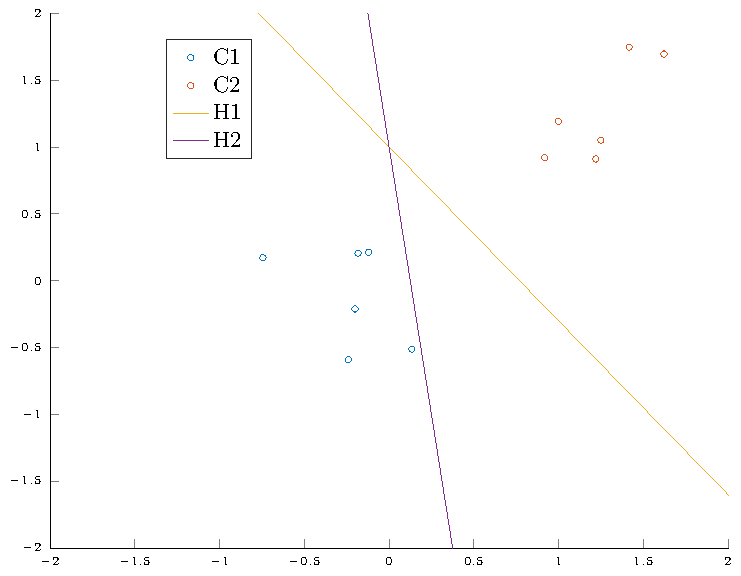
\includegraphics[width=0.85\textwidth]{\pics/c4_pics/svm_hiperplan}
\caption{Exemplu de hiperplane de decizie}
\label{fig:svm_hiper}
\end{figure}

Așa cum se poate observa în figura de mai sus setul de date este format din vectori bidimensionali structurați în două clase C1 și C2. H1 reprezintă hiperplanul optim de separație între cele două clase deoarece oferă cel mai mult spațiu între vectorii de suport iar H2 reprezintă un hiperplan de separație care neoptim din cauza aproprierii prea mari dintre el și exemplele de la clasa C1.

După cum se poate observa problema găsirii hiperplanului de separație constrânge ca datele ce se doresc a fi clasificate trebuie să fie liniar separabile \cite{svmbook}. În schimb există de asemenea modalități de a putea reprezenta în mod eficient și seturi de date cu neliniarități puternice, anume folosirea unui kernel i.e. o funcție care să transforme spațiul datelor de intrare într-un nou spațiu care să confere mai multe informații pentru clasificare. În abordarea lucrării de față vom folosi algoritmul SVM liniar.

\subsection{Problema de optimizare SVM}

Având un set de date $S={(\mathbf{x}_i, y_i)}$ unde $y_i \in {-1, 1}$ reprezintă clasa în care se află vectorul $mathbf{x}_i \in \mathbb{R}^n$, se dorește să se găsească hiperplanul de separație de 
"margine maximă":

\begin{equation}
    w \cdot \mathbf{x} - b = 0
\label{eq:svm_eq}
\end{equation}

unde $w$ reprezintă vectorul normal care definește hiperplanul de separație iar $b$ reprezintă coeficientul de compensare

Clasificarea cu SVM se realizează analizând semnul rezultatului $p = \mathbf{w} \cdot \mathbf{x} - b$

\begin{itemize}
    \item dacă $p < 0$ atunci exemplul $x$ aparține clasei -1
    \item dacă $p \geq 0$ atunci exemplul $x$ aparține clasei 1
\end{itemize}

Pentru seturi de date care nu sunt liniar separabile se folosește funcția de cost \eqref{eq:hinge}, scopul ei fiind să asigure distanța cât mai mare de separație între cele două clase.

Astfel problema de optimizare pentru SVM este dată de minimizarea costurilor pentru fiecare exemplu dat:

\begin{equation}
    \min_{w} \frac{1}{n} \sum_{i=1}^{n} max(0, 1 - y_{i}(w\cdot x_i - b)) + C||w||^2
    \label{eq:svm_opt}
\end{equation}

Introducând variabila $\zeta=max(0, 1 - y_{i}(w\cdot x_{i} - b))$ putem rescrie problema de optimizare:

\begin{subequations}
\begin{alignat}{2}
% &\!\min_{\alpha \in \mathbb{R}^n}        &\qquad& \sum_{j} \alpha_{j} \label{eq:optProb}\\
 &\!\min_{w} &  \frac{1}{n} \sum_{i=1}^{n} \zeta_{i} + C||w||^2 \label{eq:svm_opt} \\
&\text{s.l.:} &  y_{i}(w\cdot x_{i} -b) \geq 1- \zeta_i \label{eq:constr}
\end{alignat}
\label{eq:opt_problem}
\end{subequations}
Avantajul este că pentru rezolvarea acestei probleme există solvere de programare pătratică foarte performante, care întrebuințează diferite metode ale metodei gradientului.

\subsection{Motivația alegerii SVM}
Unul dintre motivele pentru care am ales acest algoritm a fost faptul că există numeroase pachete de Python care implementează atât solvere eficiente pentru problema de optimizare cât și o bibliotecă bogată și extrem de bine documentată pentru extrem de multe metode de preprocesare și algoritmi de învățare automată, precum SciKit-Learn \cite{scikit-learn} \cite{sklearn_api}.

De asemenea fiind un algoritm liniar simplu există șanse foarte mici să apară fenomenul de supra estimare \textit{overfitting} prin care modelul ales nu numai că învață trendul setului de date, dar și zgomotul de care acesta este afectat. O exemplificare a acestui fenomen este dată în figura următoare unde se compară un model simplu de gradul 1 cu un model mai complex de gradul 15:

\begin{figure}[H]
\centering
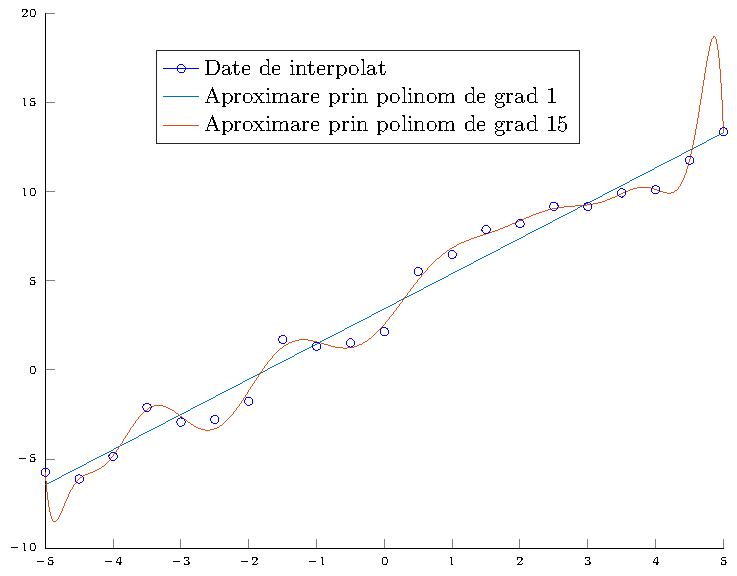
\includegraphics[width=0.85\textwidth]{\pics/c4_pics/overfitting_example}
\caption{Aproximări prin regresie liniară}
\label{fig:svm_hiper}
\end{figure}

\section{Definirea performanțelor}
Pentru un set de date $S = \{(x_i, y_i) | i = \overline{1,n}\}$ putem să evaluăm performanțele clasificatorului comparând rezultatele adevărate $y_i$ cu predicția acestuia $y_{pi}$. Ca limbaj vom considera că un exemplu selectat de clasificator va reprezenta un nod în care este prezis un defect. Astfel putem să definim următoarele:
\begin{itemize}
    \item adevărat pozitiv (TP) $y_i = y_{pi} = 1$
    \item adevărat negativ (TN) $y_i = y_{pi} = -1$
    \item fals pozitiv (FP) $y_i = -1 ~\text{și}~ y_{pi} = 1$
    \item fals negativ (FN) $y_i = 1 ~\text{și}~ y_{pi} = -1$
\end{itemize}

Iar pe baza acestora putem defini metrici precum:

Acuratețea reprezintă raportul de obiecte prezise corect din totalul de exemple:
\begin{equation}
    AC = \frac{TP + TN}{TP + TN + FP + FN}
\end{equation}

Precizia, arată câte din rezultatele selectate sunt relevante:
\begin{equation}
    P = \frac{TP}{TP + FP}
\end{equation}

Sensibilitatea, denumită și rata de retragere, raportul dintre nodurile selectate și totalul nodurilor în care există un defect:
\begin{equation}
    S = \frac{TP}{TP + FN}
\end{equation}

\section{Rezultate preliminare folosind toți senzorii}

Considerând acum setul de date pentru un algoritm liniar SVM vectorii $x_i$ vor fi reprezentați de mediile reziduurilor pe intervalul staționar, deci $x_i \in \mathbb{R}^{31}$, iar $y_{i} = \overline{1..31}$ reprezintă clasa în care poate fi situat un defect.

Setul de date a fost obținut prin considerarea a două mulțimi de defecte \cite{irofti2017dictionary}:
\begin{itemize}
    \item pentru setul de antrenare avem valori impare pentru emițător între 1 și 31
    \item pentru setul de testare avem valori pare pentru emițător între 1 și 31
\end{itemize}

Astfel rulând câte o simulare pentru fiecare nod și valoare a emițătorului ajungel a un set de antrenare $\mathbf{X}_{train} \in \mathbb{R}^{496\times 31}$ și un set de testare $\mathbf{X}_{test} \in \mathbb{R}^{465\times 31}$ pentru fiecare dintre acestea vând seturile de clase $y_{train} \in \mathbb{N}^{496}$ și $y_{test} \in \mathbb{N}^{465}$

Partea de antrenare a modelului se realizează prin folosirea unui obiect de tip SVC \textit{Support Vector Classifier} din toolkit-ul SciKit-Learn. Având ca parametru de regularizare C = 10 și kernelul liniar am obținut următoarele rezultate pe setul de testare:

\begin{table}[h]
\centering
\begin{tabular}{ |p{3cm}|p{3cm}|p{3cm}|}
\hline
Acuratețe & Precizie & Sensibilitate\\
 \hline
0.94    &  0.98     & 0.94 \\
 \hline
\end{tabular}
\caption{Metrici medii pe setul de antrenare plin}
\label{tbl:full_sensor_results}
\end{table}


\section{Selecția de senzori folosind Eliminarea recursivă de caracteristici}
Amintind de metoda de selecție a senzorilor de la secțiunea \ref{sec:sensor_selection} putem să folosim mașinile cu vectori suport pentru a ordona nodurile în ordinea importanțelor la procesul de clasificare. Aici descriem algoritmul de eliminare recursivă a caracteristicilor \textit{Recursive Feature Ellimination}. Procesul se bazează pe faptul că cele mai importante caracteristici din vectorii de intrare ale SVM-ului au ponderile cele mai mari. Astfel pentru un clasificator binar format din perechea $(w, b)$ cea mai puțin importantă caracteristică este dată de relația \cite{RFE_PAPER}: 
\begin{equation}
    arg\min_{i} ~ w
\end{equation}

Pentru a putea clasifica cele 31 de defecte, vom avea nevoie de 31 de clasificatoare de tipul \textit{One vs All}, iar ponderile pentru o astfel de problemă vor fi o matrice $mathbf{\textit{W}} \in \mathbb{R}^{n_{c}-1, n_{j}}$, unde $n_c$ reprezintă numărul de defecte iar $n_j$ reprezintă numărul de noduri folosiți pentru clasificare.

Pentru a afla scorul fiecărui nod în procesul de clasificare vom suma absolut matricea $\mathbf{W}$ pe coloane, deci:
\begin{equation}
    scor(k) = \sum_{i=1}^{n_c} |W_{ik}|
    \label{eq:scores}
\end{equation}

\paragraph{Algoritmul RFE} \mbox{} \\

Algoritmul de eliminare recursivă a caracteristicilor este descris în continuare:
\begin{algorithm2e}
\caption{Eliminarea recursivă a caracteristicilor}
\label{alg:rfe}
\KwIn{$S_{train} =\{(x_i, y_i) | i = \overline{1,n}\}$}
$C \leftarrow$ mulțimea curentă de caracteristici\;
$N_{cp} \leftarrow$ număr de caracteristici de păstrat\;
\While{$|C| > N_{cp}$} {
    antrenează clasificatorul cu caracteristicile din $C$\;
    calculează scorurile cu formula \eqref{eq:scores}\;
    elimină din mulțimea $C$ caracteristica cu scorul cel mai mic
}
\end{algorithm2e}

La finalul acestui proces mulțimea $C$ va conține $N_{cp}$ noduri care au cea mai puternică contribuție la procesul de clasificare.

\section{Rezultate folosind senzorii selectați}

Pentru a testa metoda de selecție a senzorilor am fixat un spectru pentru parametrul $N_{cp} = \{1, 4, 6, 10\}$ 

\begin{table}
    \centering
    \begin{tabular}{|c|c|c|}
    \hline
        $N_{cp}$ & Senzori selectați & Acuratețe \\
        \hline
        1 & $11$ & 64\% \\
        \hline
        4 & $10, 11, 25, 27$ & $89.6\%$\\
        \hline
        6 & $10, 11, 16, 25, 27, 28$ & $93.3\%$\\
        \hline
        10 & $ 9, 10, 11, 12, 16, 20, 25, 27, 28, 29 $ & $94.14\%$ \\
        \hline
    \end{tabular}
    \caption{Performanțele clasificării cu senzorii selectați de RFE}
    \label{tab:rfe_selected_sensors}
\end{table}

În figura următoare este reprezentată performanța fiecărui nod în procesul de clasificare:

\begin{figure}[H]
\centering
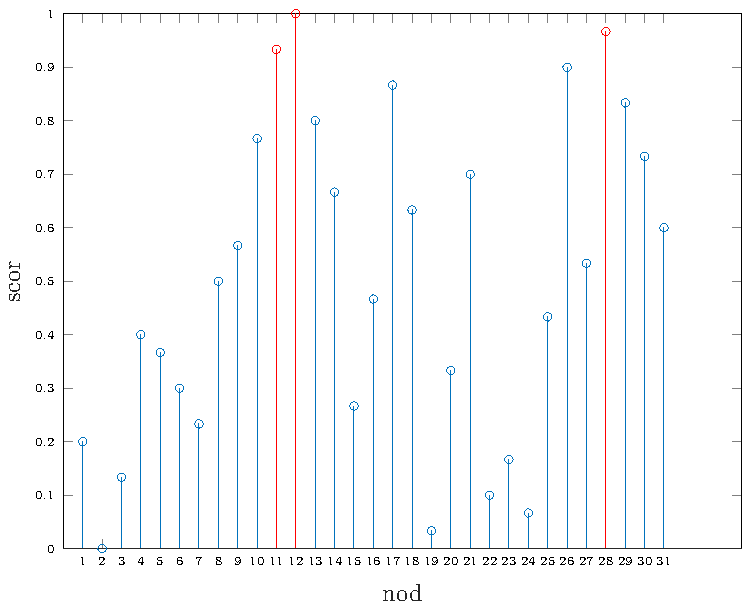
\includegraphics[width=0.85\textwidth]{\pics/c4_pics/selected_sensors}
\caption{Scorul RFE}
\label{fig:rfe_score}
\end{figure}

După cum se vede în figura \ref{fig:rfe_score} și în tabelul \ref{tab:rfe_selected_sensors} cei mai importanți senzori sunt cei reprezentați cu roșu și aduc cea mai puternică contribuție la performanțele procesului de clasificare.

\paragraph{Comparație între MSC și RFE} \mbox{} \\ 
Având în vedere că algoritmul RFE poate fi parametrizat pentru a putea selecta un anumit număr de senzori $N_{cp}$ problema MSC nu impune o constrângere explicită asupra numărului de senzori selectați, pentru a putea modifica acest număr este nevoie să considerăm modificarea limitei de sensibilitate a senzorilor pentru calcularea matricei $\mathbf{M}$ \eqref{eq:binary_matrix}

\begin{figure}[H]
\centering
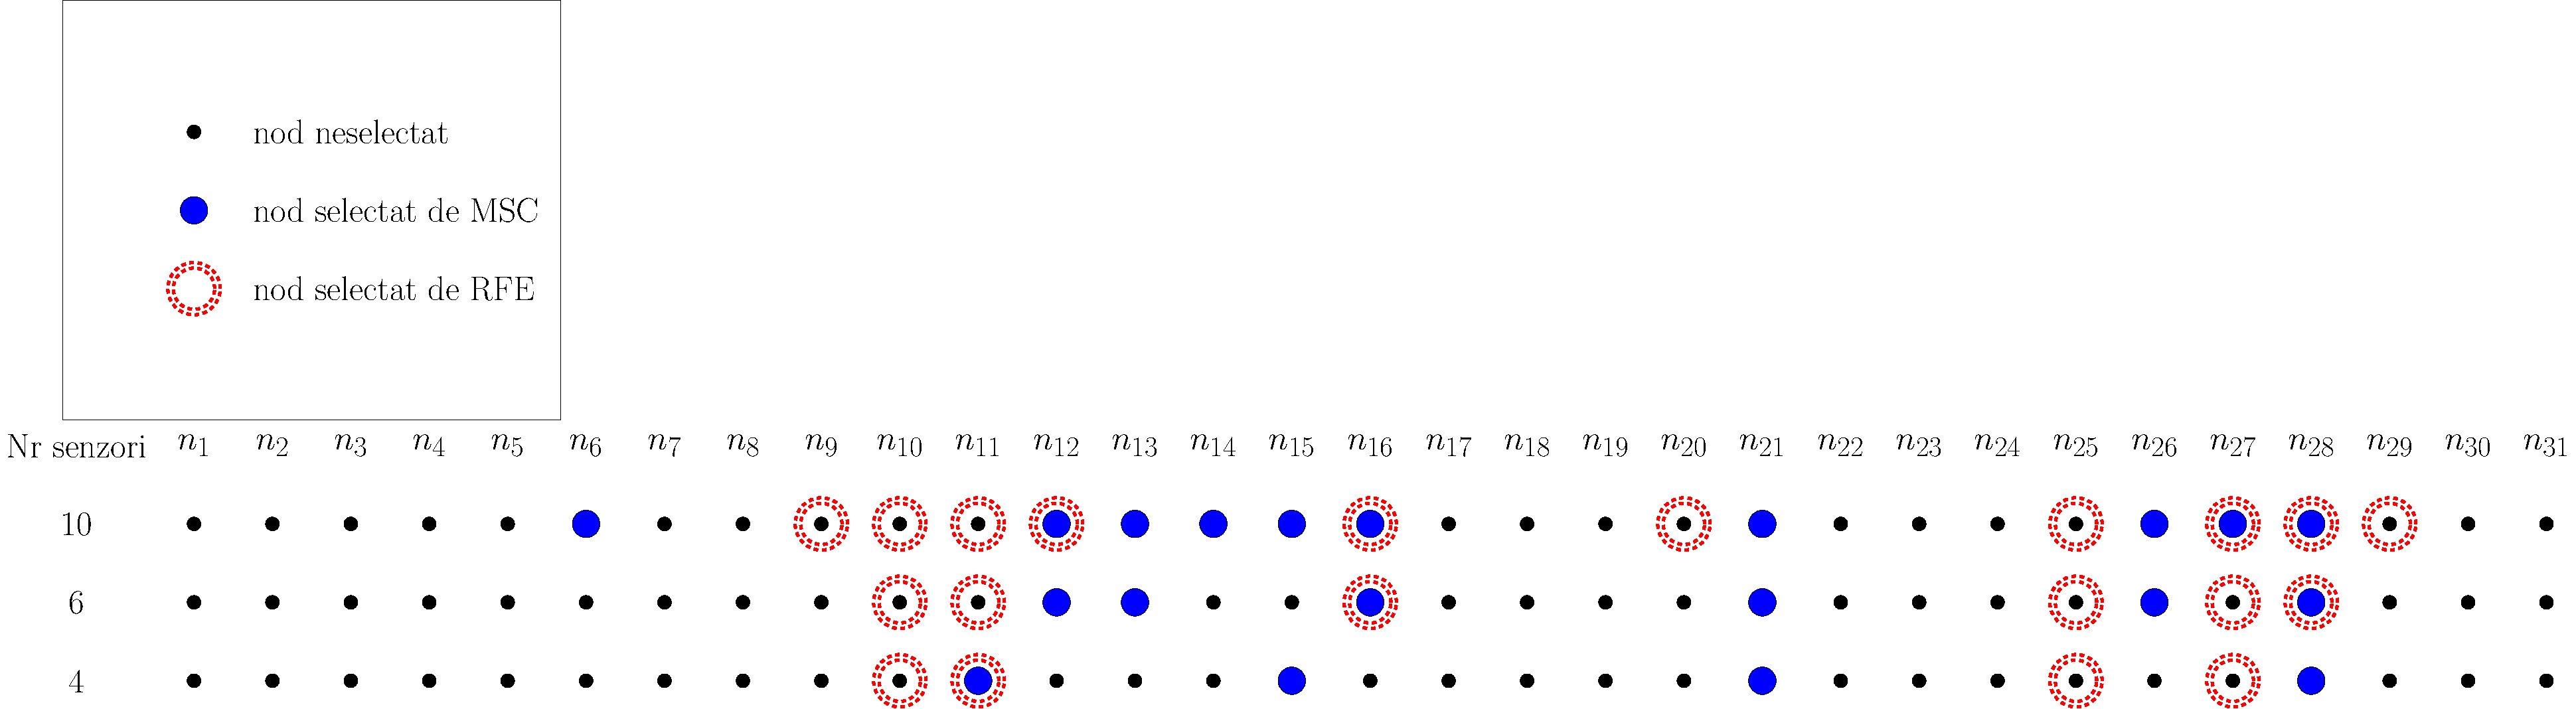
\includegraphics[width=0.85\textwidth]{\pics/c4_pics/show_selected_sensors}
\caption{Comparație între senzorii aleși de  RFE și MSC}
\label{fig:rfe_vs_msc}
\end{figure}

Figura \ref{fig:rfe_vs_msc} prezintă similaritățile între senzorii aleși de cele două metode, după cum se poate observa pentru cazul în care se doresc 4 senzori, atât MSC cât și RFE aleg senzorul 11. O particulartiate a MSC este că nu asignează o importanță a nodurilor ci doar alege acele noduri care asigură îndeplinirea condițiilor impuse de problema de minimizare. De asemenea metoda eliminării de caracteristici oferă o consistență în caracteristicile alese - pe măsură ce parametrul $N_{cp}$ crește, mulțimea de senzori selectați nu pierde elemente ci este doar completată.

\begin{table}[H]
    \centering
    \begin{tabular}{|c|c|c|}
    \hline
        Nr senzori selectați & Senzori selectați & Acuratețe \\
        \hline
        4 & $10, 11, 25, 27$ & $89.69\%$ \\
        \hline
        6 & $10, 11, 16,25, 27,28 $ & $93.3\%$\\
        \hline
        10 & $9,10, 11, 12, 16, 20, 25, 27, 28, 29$ & $94\%$\\
        \hline
    \end{tabular}
    \caption{Performanțele clasificării cu senzorii selectați de MSC}
    \label{tab:msc_selected_sensors}
\end{table}